\section{Auswertung}
\label{sec:Auswertung}
\subsection{Fouriertransformation}
\label{sec:FT}

\begin{table}
	\centering
	\begin{tabular}{S[table-format=2.0] S[table-format=3.0] S[table-format=3.0] S[table-format=2.2]}
	\toprule
{$n$} & {$\frac{U_1}{n}/\:\si{\milli{\volt}}$} & {$U_n/\:\si{\milli{\volt}}$} & {Abweichung $\:/\%$}\\
	\midrule
 1 & 920 &   \minus &  \minus\\
 3 & 300 & 288 &  4\\
 5 & 170 & 168 &  1\\
 7 & 116 & 112 &  4\\
 9 &  86 &  80 &  8\\
11 &  64 &  56 & 14\\
	\bottomrule
	\end{tabular}
	\caption{Fourieranalyse der Rechteckspannung.}
	\label{tab:FA_RE}
\end{table}
 
\begin{table}
	\centering
	\sisetup{table-format=2.3}
	\begin{tabular}{S[table-format=2.0] S[table-format=3.0] S[table-format=3.1] S[table-format=1.2] }
	\toprule
	{$n$} & {$\frac{U_1}{n²}/\:\si{\milli\volt}$} & {$U_n/\:\si{\milli\volt}$} & {Abweichung $\:/\%$}\\
	\midrule
 1 & 580 & \minus  &  \minus\\
 3 &  63 &  61.6 & 2.3\\
 5 &  21 &  20.8 & 1.0\\
 7 &  10 &  10.4 & 3.9\\
 9 &   6 &   5.6 & 7.1\\
11 &   4 &   4.0 & 0.0\\
	\bottomrule
	\end{tabular}
	\caption{Fourieranalyse der Dreiecksspannung.}
	\label{tab:FA_DE}
\end{table}



\begin{table}
	\centering
	\sisetup{table-format=2.3}
	\begin{tabular}{S[table-format=2.0] S[table-format=3.0] S[table-format=3.1] S[table-format=1.0] }
	\toprule
	{$n$} & {$\frac{U_1}{n}/\:\si{\milli{\volt}}$} & {${U_n}/\:\si{\milli\volt}$} & {Abweichung $\:/\%$}\\
	\midrule
 1 & 460 & \minus   &\minus\\
 2 & 230 & 224 & 3\\
 3 & 152 & 144 & 6\\
 4 & 112 & 112 & 0\\
 5 &  88 &  88 & 0\\
 6 &  74 &  74 & 0\\
 7 &  64 &  64 & 0\\
 8 &  56 &  56 & 0\\
 9 &  50 &  48 & 4\\
10 &  44 &  46 & 5\\
11 &  40 &  40 & 0\\
	\bottomrule
	\end{tabular}
	\caption{Fourieranalyse der Sägezahnspannung.}
	\label{tab:FA_SZ}
\end{table}

Die Tabellen \ref{tab:FA_RE},\ref{tab:FA_DE} und \ref{tab:FA_SZ} enthalten die gemessenen Amplituden ${U_n}$ der $n$-ten Oberschwingung. 
Nach Gleichung \eqref{eq:koeff2} wurden in der Versuchsvorbereitung die Koeffizienten $a_n$, $b_n$ der verschiedenen Spannungsformen berechnet. Es gilt
\begin{align} 
\text{Rechteck}:\quad & a_n=0, & b_n=\frac{4 U_0}{\pi n}
\label{koeff1}
\\
\text{Sägezahn}:\quad & a_n=0,  & b_n={(-1)}^{n+1}\frac{2U_0}{\pi n}
\label{koeff2}\\
\text{Dreieck}: \quad & a_n=\frac{8U_0}{n²\pi²},  & b_n=0,\label{koeff3}
\end{align}
mit Rechteck- und Sägezahnspannung als gerade Funktionen; die Dreieckspannung ist ungerade.
Nach diesen Formeln wird die theoretisch erwartete Amplitude $\frac{U_1}{n}$ berechnet, in dem die erste gemessene Amplitude als gegeben vorausgesetzt wird und anschließend durch $n$ bzw. $n²$ geteilt wird, um die restlichen Theoriewerte zu erhalten. Die Abweichung zwischen Messung und Theorie ist ebenfalls angegeben.
\begin{figure}
	\centering
		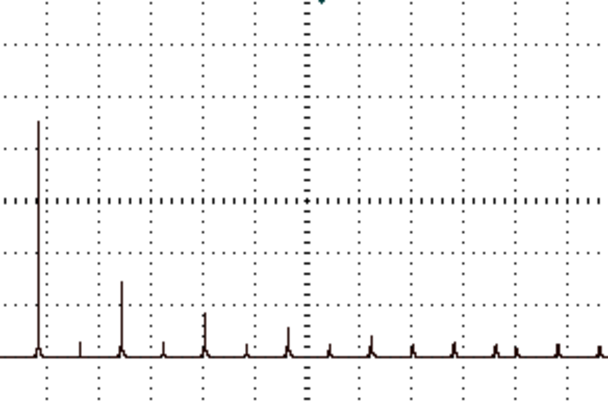
\includegraphics[width=0.7\textwidth]{Bilder/FT_RE2.pdf}		
\caption{Fourieranalyse der Rechteckspannung.}
	\label{fig:FT_RE}
\end{figure}


\begin{figure}
	\centering
		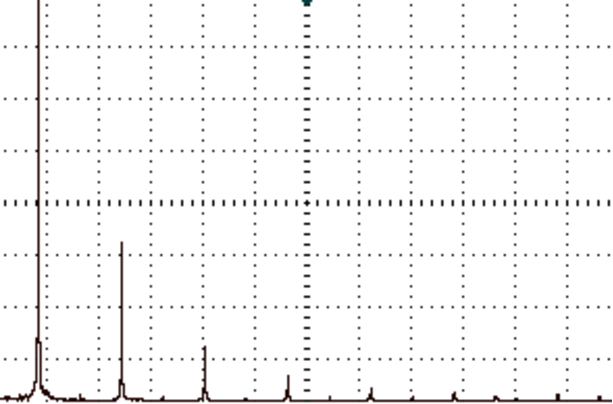
\includegraphics[width=0.7\textwidth]{Bilder/FT_DE2.pdf}		
\caption{Fourieranalyse der Dreieckspannung.}
	\label{fig:FT_DE}
\end{figure}


\begin{figure}
	\centering
		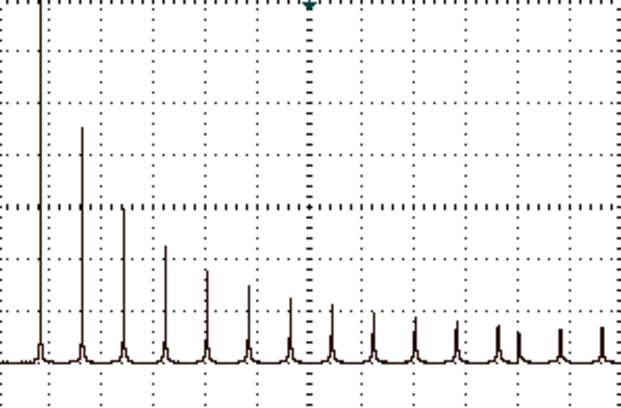
\includegraphics[width=0.7\textwidth]{Bilder/FT_SZ.pdf}		
\caption{Fourieranalyse der Sägezahnspannung.}
	\label{fig:FT_SZ}
\end{figure}

In den Abbildungen \ref{fig:FT_DE} und \ref{fig:FT_RE} werden die Amplituden der Koeffizienten dargestellt. Nach Gleichung  \eqref{koeff1} und \eqref{koeff2} sollen alle geraden Koeffizienten wegfallen. Verlgeicht man die Theorie mit den Abbildungen fällt auf, dass dies -- bedingt durch die verwendeten Bauteile in der Messung -- nicht der Fall ist. Es treten Spannungen $U\geqslant0\,\si\volt$ auf Diese Abweichungen lassen sich für größere $n$ nur schwierig von den Amplituden der ungeraden Koeffizienten unterscheiden.
Die Abbildung \ref{fig:FT_SZ} stimmt gut mit der Theorie überein, weist jedoch einen messtechnisch bedingten Fehler auf. Der Abstand zwischen dem 12. und 13. Peak weicht von der Größe der anderen Abstände ab. Bei Rechteck- und Dreieckspannung tritt der gleiche Fehler auf, was aber aufgrund der Peak-Höhe nicht direkt zu erkennen ist.

\subsection{Fouriersynthese}
Bei der Fouriersynthese sollen die in Kapitel \ref{sec:FT} untersuchen Schwingungen aus einzelnen Koeffizienten hergestellt werden. Dazu werden die Amplituden der verschiedenen Oberschwingungen am Oberwellengenerator eingestellt und die Phase so geändert, dass die auf dem Oszilloskopbildschirm dargestellte Summenspannung dem gewählten Spannungsverlauf entspricht. In Tabelle \ref{tab:FS} sind die Amplituden der unterschiedlichen Oberwellen für Rechteck-, Dreieck- und Sägezahnspannung aufgetragen.

\begin{table}
	\centering
	\begin{tabular}{cccc}	
	\toprule
\multicolumn{1}{c}{n} & \multicolumn{3}{c}{$U_n\:/\si{\milli{\volt}}$}\\
	{} & {Rechteck} & {Sägezahn} & {Dreieck}\\
	\midrule
 1 & 634.8  & 634.8  & 634.80\\
 2 &   0    & 318.00 &   0\\
 3 & 216.73 & 212.00 &  70.72\\
 4 &   0    & 159.76 &   0\\
 5 & 130.20 & 127.65 &  25.48\\
 6 &   0    & 106.45 &   0\\
 7 &  92.90 &  91.20 &  13.27\\
 8 &   0    &  79.49 &   0\\
 9 &  72.08 &  70.55 &  7.95\\
	\bottomrule
	\end{tabular}
	\caption{Fouriersynthese drei verschiedener Spannungen.}
	\label{tab:FS}
\end{table}






\begin{figure}
	\centering
		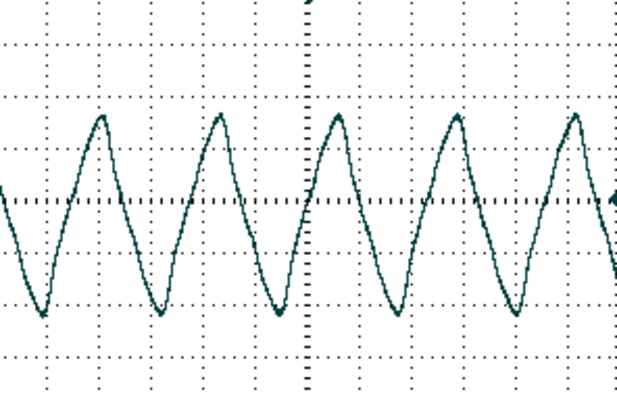
\includegraphics[width=0.7\textwidth]{Bilder/1-9_DE.pdf}		
\caption{Fouriersynthese der Dreiecksspannung.}
	\label{fig:1-9_DE}
\end{figure}

In Abbildung \ref{fig:1-9_DE} ist die synthetisierte Dreieckspannung abgebildet. Die Flanken sind nicht gerade, sondern weisen Schwingungsbäuche auf. Die Spannungsspitzen sind abgerundet. Trotzdem ist die maßgebliche, dreieckige Form gut erkennbar.

\begin{figure}
	\centering
		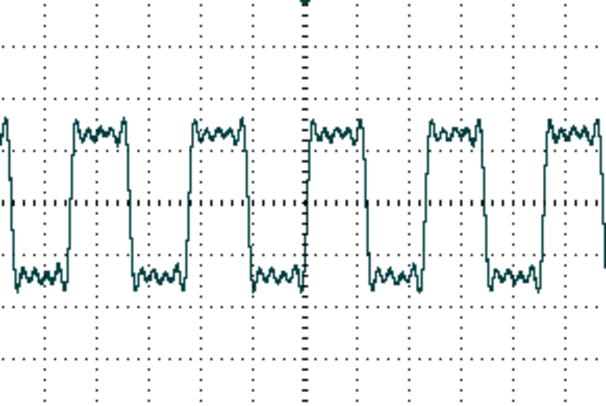
\includegraphics[width=0.7\textwidth]{Bilder/1-9_RE.pdf}		
\caption{Fouriersynthese der Rechteckspannung.}
	\label{fig:1-9_RE}
\end{figure}
Die Rechteckspannung ist ebenfalls gut zu erkennen, weist aber -- hauptsächlich an den Maximalwerten der Spannung vorzufindende -- Abweichungen auf. 

\begin{figure}
	\centering
		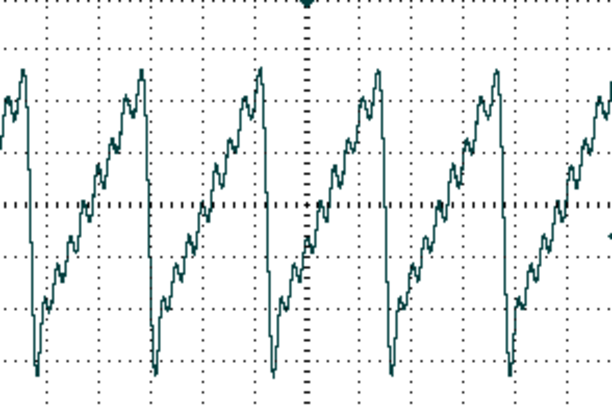
\includegraphics[width=0.7\textwidth]{Bilder/1-9_SZ.pdf}		
\caption{Fouriersynthese der Sägezahnspannung.}
	\label{fig:1-9_SZ}
\end{figure}
Abbildung \ref{fig:1-9_SZ} zeigt die Sägezahnspannung. Diese unterscheidet sich vom idealen Aussehen durch nicht ganz senkrecht abfallende Flanken und Schwingungen an steigenden Flanken.

Die relativ starken Abweichungen werden erzeugt, da die Fourier-Synthese nach $n=10$ Oberschwingungen abgebrochen wird. Durch größere Werte für $n$, sowie noch genaueres einstellen der Phasen kann der Fehler weiter minimiert werden.
